\documentclass[twocolumn]{aastex63}

% typography
\usepackage[T1]{fontenc}

\setlength{\parindent}{1.\baselineskip}
\newcommand{\acronym}[1]{{\small{#1}}}
\newcommand{\package}[1]{\textsl{#1}}
\newcommand{\gaia}{\textsl{Gaia}}
\newcommand{\pans}{\textsl{Pan-STARRS}}

\newcommand{\apw}[1]{{\color{blue} APW: #1}}
\newcommand{\kpc}{\ensuremath{\textrm{kpc}}}
\newcommand{\kms}{\ensuremath{\textrm{km}\,\textrm{s}^{-1}}}
\newcommand{\masyr}{\ensuremath{\textrm{mas}\,\textrm{yr}^{-1}}}
\newcommand{\feh}{\ensuremath{\textrm{[Fe/H]}}}
\newcommand{\afe}{\ensuremath{\textrm{[$\alpha$/Fe]}}}
\newcommand{\changes}[1]{{\textbf{#1}}}

% aastex parameters
% \received{not yet; THIS IS A DRAFT}
%\revised{not yet}
%\accepted{not yet}
% % Adds "Submitted to " the arguement.
% \submitjournal{ApJ}
\shorttitle{spur spec}
\shortauthors{bonaca et al.}

%@arxiver{}
\usepackage{amsmath}

\begin{document}\sloppy\sloppypar\raggedbottom\frenchspacing % trust me

\title{Spectroscopy of the GD-1 spur}

\correspondingauthor{Ana Bonaca}
\email{ana.bonaca@cfa.harvard.edu}

\author[0000-0002-7846-9787]{Ana Bonaca}
\affil{Center for Astrophysics | Harvard \& Smithsonian, 60 Garden Street, Cambridge, MA 02138, USA}

\author{collaborators}
% \affil{Center for Astrophysics | Harvard \& Smithsonian, 60 Garden Street, Cambridge, MA 02138, USA}


% \author[0000-0002-1590-8551]{Charlie Conroy}
% \affil{Center for Astrophysics | Harvard \& Smithsonian, 60 Garden Street, Cambridge, MA 02138, USA}
% 
% \author[0000-0003-0872-7098]{Adrian~M.~Price-Whelan}
% \affil{Department of Astrophysical Sciences, 4 Ivy Lane, Princeton University, Princeton, NJ 08544, USA}
% 
% \author[0000-0003-2866-9403]{David W. Hogg}
% \affiliation{Center for Cosmology and Particle Physics,
% Department of Physics,
% New York University}
% \affiliation{Center for Data Science,
% New York University}
% \affiliation{Max-Planck-Institut f\"ur Astronomie, Heidelberg}
% \affiliation{Flatiron Institute, Simons Foundation}

\begin{abstract}\noindent % trust me
- gaia revealed gd1-like stars outside of the main stream
- we confirm the association kinematically and chemically using high-resolution, MMT/Hectochelle spectroscopy
- at fixed location along the stream, the median radial velocity offset of the spur with respect to the main stream is smaller than $0.5\,\kms$, comparable to the measurement uncertainty
- the radial velocity dispersion is low in both components, $\sigma_{V_r}\lesssim1.5\,\kms$, and consistent with a globular cluster origin.
- gd-1 stars are metal-poor, $\feh\approx-2.1$, with little dispersion, but spread a 0.5\,dex range in $\afe$ abundance.
- implication for the spur formation
% with radial velocities, and chemically with feh and afe
% - hectochelle

% In simple models of the Milky Way, tidally disrupting satellites produce long and thin---nearly one-dimensional---stellar streams.
% Using astrometric data from the Gaia second data release and photometry from the Dark Energy Survey, we demonstrate that the Jhelum stream, a stellar stream in the inner halo, is a two-dimensional structure.
% The spatial distribution of highly probable Jhelum members reveals a dense thin component and an associated diffuse, spatially offset component.
% These two spatial components have indistinguishable proper motions (at $\sigma\sim1\,\rm mas\,yr^{-1}$ level) and a similar ratio of blue straggler to blue horizontal branch stars, which indicates a common origin for the two components.
% The best-fit orbit to the narrow component (pericenter $8\,\rm kpc$, apocenter $24\,\rm kpc$), however, does not explain the wide component of the Jhelum stream.
% On the other hand, an older orbital wrap of Jhelum's orbit traces the Indus stream, indicating a possible connection between these two structures and additional complexity in Jhelum's formation.
% Substructure in the Jhelum progenitor or precession of its tidal debris in the Milky Way potential may explain the observed structure of Jhelum.
% Future spectroscopic data will enable discrimination between these ``nature'' and ``nurture'' formation scenarios.
% Jhelum adds to the growing list of cold stellar streams that display complex morphologies and promise to reveal the dynamical history of the Milky Way.
\end{abstract}

\keywords{%
stars:~kinematics~and~dynamics
  ---
Galaxy:~halo
  ---
Galaxy:~kinematics~and~dynamics
}

\section{Introduction}
\label{sec:intro}

% The spread in proper motions indicates GD-1 has a low velocity dispersion \citep[$\lesssim1.5\,\kms$,][]{malhan2019}, .


\section{Spectroscopy}
\label{sec:spec}

\begin{figure*}
\begin{center}
\includegraphics[width=0.9\textwidth]{spectra.pdf}
\end{center}
\caption{
}
\label{fig:spectra}
\end{figure*}

We observed the GD-1 stellar stream using MMT/Hectochelle multi-object spectrograph \citep{szentgyorgyi2011}.
Focusing on the perturbed area at $\phi_1\approx-40^\circ$ \citep[$\phi_{1,2}$ are coordinates oriented along and perpendicular to GD-1, respectively;][]{koposov2010}, we targeted 4 fields in the main stream, and 4 fields in the lower-density spur (labeled in Figure~\ref{fig:spectra}, top).
Using the Gaia--PanSTARRS-1 cross-matched catalog, we selected retrograde stars as science targets, first prioritizing stars on the GD-1 main sequence, and then its red giant branch \citep[see][]{pwb}.
On average, we dedicated $\gtrsim170$ fibers to science targets per field, for a total of 1409 science spectra.
Up to 40 of the remaining fibers were used to estimate the sky emission.
We used the \texttt{RV31} filter covering the Mg~b triplet and observed each field for 2.25~hours (except for field 3 which was observed for 2~hours due to scheduling constraints).
With $3\times2$ spectral and spatial binning of the CCD pixels, we achieved a signal-to-noise ratio $S/N\approx2$ at $g=20$ and an effective resolution $R\approx32,000$.
Representative spectra in the 90th, 50th, and 10th percentile of $S/N$ are shown in rows 2 through 4 of Figure~\ref{fig:spectra}.

The 2D spectra were reduced by \package{HSRED}~v2.1\footnote{\url{https://bitbucket.org/saotdc/hsred/}}.
This pipeline flat-fields, wavelength-calibrates with respect to ThAr lamp spectra, extracts 1D spectra and subtracts the sky emission.
We then used the \package{MINESweeper} code \citep{cargile2019} to forward-model the processed 1D spectra and infer stellar parameters, including radial velocities, [Fe/H] and [$\alpha$/Fe] abundances.
The best-fit solutions for the spectra in Figure~\ref{fig:spectra} are overplotted in orange, while the residuals are shown in gray at the bottom.
Radial velocities are measured to better than $\lesssim1\,\kms$ (median $\sigma_{V_r}=0.3\,\kms$), while typical uncertainties for [Fe/H] and [$\alpha$/Fe] are $0.07$\,dex and $0.05$\,dex, respectively.
Despite the sub-$\kms$ statistical precision, sky-emission lines show variations of $\approx1\,\kms$ across the two camera chips and between different exposures.
Our overall kinematic precision is therefore systematics-dominated at $\approx1\,\kms$, comparable to that typically achieved with Hectochelle \citep[e.g.,][]{caldwell2017}, and sufficient to resolve the GD-1 internal dispersion \citep{malhan2019}.

\section{Stream membership}
\label{sec:membership}

\begin{figure*}
\begin{center}
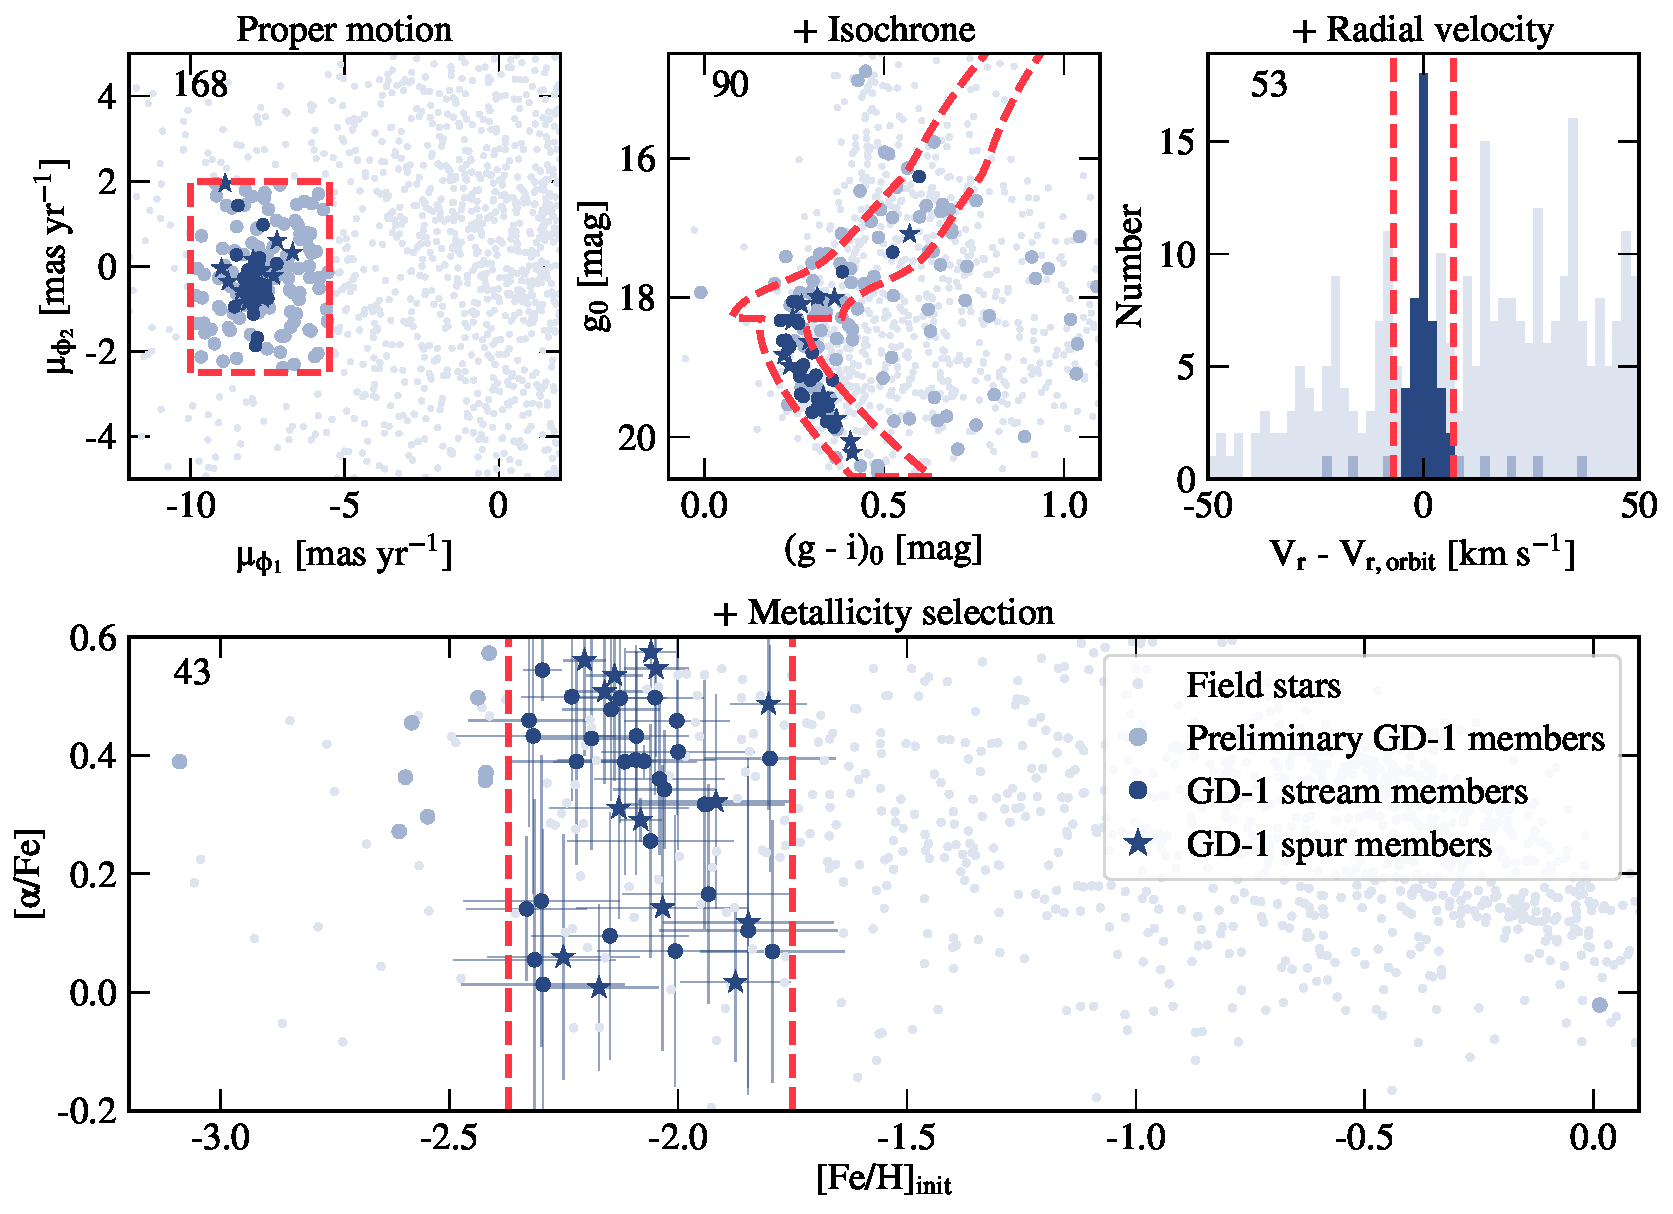
\includegraphics[width=0.99\textwidth]{members.pdf}
\end{center}
\caption{
}
\label{fig:members}
\end{figure*}

Since GD-1 is a retrograde, metal-poor stream, membership selection based on \gaia\ proper motions \citep{gdr2} and de-reddened \pans\ photometry \citep{sfd, ps1} is very efficient \citep[e.g.,][]{pwb}.
The left panel of Figure~\ref{fig:members} shows the color-magnitude diagram (CMD) of all targeted stars: those with GD-1-like proper motions are dark blue ($-9<\mu_{\phi_1}/\masyr<-4.5$ and $-1.7<\mu_{\phi_2}/\masyr<1$, corrected for solar reflex motion following \citealt{pwb}), and the filler retrograde stars are light blue.
We further consider stars close to the $\textrm{[Fe/H]}=-1.5$, 12.6\,Gyr isochrone at 7.8\,kpc \citep{choi2016} as more likely GD-1 members.
The isochrone selection box (dashed pink) is tighter around the GD-1's main sequence where the contrast with respect to the Milky Way field is higher, and more generous at the red giant branch, allowing for uncertainties in the adopted isochrone.
A total of 97 stars satisfy the proper motion and CMD selection criteria.

Most of these likely members have small radial velocity offsets from the GD-1's orbit (Figure~\ref{fig:members}, middle panel).
% - refit only 4 stream fields, yield 6d position in the gala fiducial potential:
We used the orbital solution from \citet{pwb}, which is $\Delta V_r\approx10\,\kms$ offset from Hectochelle radial velocities, so we further select 61 more likely members with velocity offsets $-20 < \Delta V_r / \kms < -1$.
Stars from both the main stream and the spur satisfy these criteria, indicating that the spur is dynamically associated with GD-1.
We explore this connection in more detail in Section~\ref{sec:kinematics}.
% 
Thus selected GD-1 members are predominantly metal-poor, as found by \citet{malhan2019}, so we adopt $-2.8<\feh<1.9$ as our final criterion for GD-1 membership (Figure~\ref{fig:members}, right).
% This produces a sample of 54 most likely GD-1 stars.
Although wide, this metallicity selection removes only two kinematically identified members for a final sample of 54 most likely GD-1 stars.

In addition to determining membership, chemical abundances of stream stars are the best way to differentiate between a globular cluster and a dwarf galaxy origin in the absence of a progenitor.
Abundance spreads are typically a signature of a dwarf galaxy origin \citep[e.g.,][]{willman2012}, however, globular clusters observed with the same instrumental setup as used here (although at a higher signal-to-noise ratio) show spreads on the order of $\approx0.05-0.1$\,dex \citep{cargile2019}.
The standard deviations in $\feh$ and $\afe$ of GD-1 members are 0.17\,dex and 0.16\,dex, respectively, and are almost entirely accounted for by the measurement uncertainties (median $\sigma_\feh=0.16$\,dex, $\sigma_\afe=0.14$\,dex, larger than our typical target since most of the members are faint main-sequence stars).
These data suggest that GD-1 is likely a disrupted globular cluster, as previously inferred from its narrow width \citep[e.g.,][]{grillmair2006} and cold kinematics \citep[e.g.,][]{malhan2019}.
% However, the median metallicity of $\feh=-2.3\pm0.2$ places GD-1 progenitor among the most metal-poor globular clusters found in the Milky Way globular.
More detailed abundances will enable an even more efficient membership selection, and a definitive classification of GD-1's progenitor.





% which is in contrast with GD-1's thin width and cold kinematics, usually interpreted as signatures of a tidally disrupted globular cluster \citep[e.g.,][]{grillmair2006,malhan2019}.

% To quantify the amount of spread in GD-1 chemical abundances, we model their distribution in the [$\alpha$/Fe] vs [Fe/H] plane as a two dimensional Gaussian.
% - likelihood, accounting for observational uncertainties
% - sampling w emcee
% - we infer intrinsic spread of $\sigma_{\mathrm{[Fe/H]}}=\pm$ and $\sigma_{[\alpha\mathrm{/Fe]}}=\pm$
% - while the feh spread is marginal, the afe is detected at xsigma, which complicates the interpretation of GD-1 as a globular cluster stream
% - globular clusters can also have a spread in Mg (cit), where most of our alpha info is coming from)
% - more detailed abundances are required to conclusively identify the nature of GD-1's progenitor, a requirement for interpreting density variations along the stream \citep[e.g.,][]{kupper}.

% - spreads typically associated w dwarf galaxy progenitors (eg, cit), but globular clusters can also have a spread in Mg (where most of our alpha info is coming from), so more detailed abundances are required to conclusively identify the nature of GD-1's progenitor
% - future: membership probability with background model, but the current selection ok for now


\section{GD-1 kinematics}
\label{sec:kinematics}


% \section{Model}
% \label{sec:model}


\section{Discussion}
\label{sec:discussion}


Acknowledgments: 
- gaia sprint
- kitp
- mpia

\bibliographystyle{aasjournal}
\bibliography{spur_rv}


\end{document}